\documentclass[../main.tex]{subfiles}

\begin{document}
\chapter{probability}


\addcontentsline{toc}{section}{Experiment}
\begin{statement}[\textbf{Experiment}]
\label{statement:Experiment}\hspace*{0pt}\par
\end{statement}
\textbf{Description}:
A list of instructions which when followed produces an outcome.
\par
{\color{magenta} \textbf{Significance}:
Anything that has some non-zero number of outcomes is an experiment.
The meaning of this is not just limited to experiments which involve physics or chemistry.
We are only concerned with the outcomes and not the inputs.
Note that, at a time only one of the several possible outcomes of an experiment can occur.
\par}
\begin{proof}Axiom.\end{proof}\par
\paragraph{0 parents} 
\paragraph{7 children} \hyperref[statement:Deterministic Experiment]{Deterministic Experiment}, \hyperref[statement:Non-deterministic Experiment]{Non-deterministic Experiment}, \hyperref[statement:Outcome Space]{Outcome Space}, \hyperref[statement:Event]{Event}, \hyperref[statement:Mutually Exclusive Events]{Mutually Exclusive Events}, \hyperref[statement:Event Space]{Event Space}, \hyperref[statement:Stochastic Experiment]{Stochastic Experiment}, 





\addcontentsline{toc}{section}{Deterministic Experiment}
\begin{statement}[\textbf{Deterministic Experiment}]
\label{statement:Deterministic Experiment}\hspace*{0pt}\par
\end{statement}
\textbf{Description}:
Let $ O_k $ represent the final outcome when an [\hyperref[statement:Experiment]{experiment}] is repeated k times, an experiment such that $ O_1, O_2, O_3, ... O_n $ are pairwise identical [\hyperref[statement:Identity]{identity}] $\forall n \in \mathbb{N} $ [\hyperref[statement:Natural Numbers]{natural numbers}] is called a deterministic experiment.
\par
{\color{magenta} \textbf{Significance}:
Can be used to represent experiments like adding two numbers.
\par}
\begin{proof}
\proofbydefinition
\end{proof}\par
\paragraph{3 parents} \hyperref[statement:Experiment]{Experiment}, \hyperref[statement:Identity]{Identity}, \hyperref[statement:Natural Numbers]{Natural Numbers}, 
\paragraph{0 children} 



\addcontentsline{toc}{section}{Non-deterministic Experiment}
\begin{statement}[\textbf{Non-deterministic Experiment}]
\label{statement:Non-deterministic Experiment}\hspace*{0pt}\par
\end{statement}
\textbf{Description}:
Let $ O_k $ represent the final outcome when an [\hyperref[statement:Experiment]{experiment}] is repeated k times, an experiment such that $ \exists (i, j) \st O_i \not\equiv O_j $ [\hyperref[statement:Identity]{identity}] is called a non-deterministic experiment.
\par
{\color{magenta} \textbf{Significance}:
Note that outcome can remain same for some repetitions of the experiement.
Can be used to represent experiments like rolling a dice.
\par}
\begin{proof}
\proofbydefinition
\end{proof}\par
\paragraph{2 parents} \hyperref[statement:Experiment]{Experiment}, \hyperref[statement:Identity]{Identity}, 
\paragraph{0 children} 



\addcontentsline{toc}{section}{Outcome Space}
\begin{statement}[\textbf{Outcome Space}]
\label{statement:Outcome Space}\hspace*{0pt}\par
\end{statement}
\textbf{Description}:
The outcome space of an [\hyperref[statement:Experiment]{experiment}] is the [\hyperref[statement:Set]{set}] of its all possible outcomes [\hyperref[statement:Universal Set]{universal set}].
\par
{\color{magenta} \textbf{Significance}:
A term to refer to all possible outcomes collectively.
\par}
\begin{proof}
\proofbydefinition
\end{proof}\par
\paragraph{3 parents} \hyperref[statement:Experiment]{Experiment}, \hyperref[statement:Set]{Set}, \hyperref[statement:Universal Set]{Universal Set}, 
\paragraph{4 children} \hyperref[statement:Event]{Event}, \hyperref[statement:Properties of probability]{Properties of probability}, \hyperref[statement:Total Probability Theorem]{Total Probability Theorem}, \hyperref[statement:Bayes Theorem]{Bayes Theorem}, 



\addcontentsline{toc}{section}{Event}
\begin{statement}[\textbf{Event}]
\label{statement:Event}\hspace*{0pt}\par
\end{statement}
\textbf{Description}:
An event $ E $ of an [\hyperref[statement:Experiment]{experiment}] is a [\hyperref[statement:Subset]{subset}] of [\hyperref[statement:Outcome Space]{outcome space}]. An event is said to have occured $ \biimpl $ $ \exists $ outcome $ \in E $ that occured.
\par
{\color{magenta} \textbf{Significance}:
The naming here is bad.
An event is nothing but a set of outcomes.
An event Q occured is equivalent to saying that the experiement's outcome was one of outcomes in Q.
That's it.
Nothing more.
The number of elements in an event can be 0, 1 or even total number of possible outcomes.
\par}
\begin{proof}
\proofbydefinition
\end{proof}\par
\paragraph{3 parents} \hyperref[statement:Experiment]{Experiment}, \hyperref[statement:Subset]{Subset}, \hyperref[statement:Outcome Space]{Outcome Space}, 
\paragraph{9 children} \hyperref[statement:Mutually Exclusive Events]{Mutually Exclusive Events}, \hyperref[statement:Event Space]{Event Space}, \hyperref[statement:Stochastic Experiment]{Stochastic Experiment}, \hyperref[statement:Probability]{Probability}, \hyperref[statement:Properties of probability]{Properties of probability}, \hyperref[statement:Independent Events]{Independent Events}, \hyperref[statement:Conditional Probability]{Conditional Probability}, \hyperref[statement:Total Probability Theorem]{Total Probability Theorem}, \hyperref[statement:Bayes Theorem]{Bayes Theorem}, 



\addcontentsline{toc}{section}{Mutually Exclusive Events}
\begin{statement}[\textbf{Mutually Exclusive Events}]
\label{statement:Mutually Exclusive Events}\hspace*{0pt}\par
\end{statement}
\textbf{Description}:
Two [\hyperref[statement:Event]{event}]s A and B of an [\hyperref[statement:Experiment]{experiment}] are mutually exclusive events $ \biimpl $ $ A \cap B \equiv \phi $ [\hyperref[statement:Null Set]{null set}].
\par
{\color{magenta} \textbf{Significance}:
For example in the experiement of throwing a dice the event of getting an even number and the event of getting an odd number are mutually exclusive events.
Note that they are not independent events, even both words are eerily similar.
Mutually exclusive mean that at max one can occur at a given time.
Independent means both can occur at the same time.
Mutually exclusive events can occur in non-stochastic experiements too.
Independent events can not occur in non-stochastic experiements.
\par}
\begin{proof}
\proofbydefinition
\end{proof}\par
\paragraph{3 parents} \hyperref[statement:Event]{Event}, \hyperref[statement:Experiment]{Experiment}, \hyperref[statement:Null Set]{Null Set}, 
\paragraph{0 children} 



\addcontentsline{toc}{section}{Event Space}
\begin{statement}[\textbf{Event Space}]
\label{statement:Event Space}\hspace*{0pt}\par
\end{statement}
\textbf{Description}:
The event space of an [\hyperref[statement:Experiment]{experiment}] is the [\hyperref[statement:Set]{set}] of all possible [\hyperref[statement:Event]{event}]s of the experiement.
\par
{\color{magenta} \textbf{Significance}:
A term to refer to all possible events collectively
\par}
\begin{proof}
\proofbydefinition
\end{proof}\par
\paragraph{3 parents} \hyperref[statement:Experiment]{Experiment}, \hyperref[statement:Set]{Set}, \hyperref[statement:Event]{Event}, 
\paragraph{2 children} \hyperref[statement:Stochastic Experiment]{Stochastic Experiment}, \hyperref[statement:Random Variable]{Random Variable}, 




\addcontentsline{toc}{section}{Stochastic Experiment}
\begin{statement}[\textbf{Stochastic Experiment}]
\label{statement:Stochastic Experiment}\hspace*{0pt}\par
\end{statement}
\textbf{Description}:
An [\hyperref[statement:Experiment]{experiment}] such that $\forall$ [\hyperref[statement:Event]{event}] $ \lambda \in $ [\hyperref[statement:Event Space]{event space}] the limiting value of the ratio
\[
\frac{\text{number-of-times-$\lambda$-occured}}{\text{number-of-repetitions}}
\]
as the number of repetitions tend to infinity, exists, is called a stochastic experiment.
\par
{\color{magenta} \textbf{Significance}:
Useful to build the concept of probability.
Note that by my definition of stochastic experiment
\begin{enumerate}[nolistsep]
    \item All deterministic experiments are stochastic experiments with probability of the only outcome being 1.
    \item Some non-deterministic experiments are stochastic experiments.
\end{enumerate}
\begin{center}
    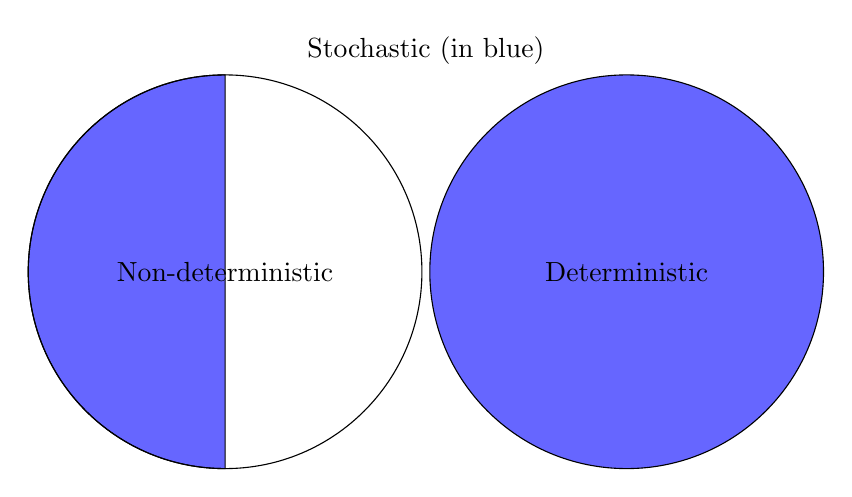
\begin{tikzpicture}
    \setlength{\parskip}{5mm}
        \draw[fill=blue!60]     (0, 0) -- (90:2.5) arc (90:270:2.5) -- cycle ;
        \draw[]                 (0, 0) circle (2.5) node {Non-deterministic};
        \draw[fill=blue!60]     (0: 5.1) circle (2.5) node {Deterministic};
        \node[anchor=south] at (current bounding box.north) {Stochastic (in blue)};
    \end{tikzpicture}
\end{center}
\par}
\begin{proof}
\proofbydefinition
\end{proof}\par
\paragraph{3 parents} \hyperref[statement:Experiment]{Experiment}, \hyperref[statement:Event]{Event}, \hyperref[statement:Event Space]{Event Space}, 
\paragraph{7 children} \hyperref[statement:Probability]{Probability}, \hyperref[statement:Properties of probability]{Properties of probability}, \hyperref[statement:Independent Events]{Independent Events}, \hyperref[statement:Conditional Probability]{Conditional Probability}, \hyperref[statement:Random Variable]{Random Variable}, \hyperref[statement:Total Probability Theorem]{Total Probability Theorem}, \hyperref[statement:Bayes Theorem]{Bayes Theorem}, 



\addcontentsline{toc}{section}{Probability}
\begin{statement}[\textbf{Probability}]
\label{statement:Probability}\hspace*{0pt}\par
\end{statement}
\textbf{Description}:
The probability of an [\hyperref[statement:Event]{event}] $ \lambda $ of a [\hyperref[statement:Stochastic Experiment]{stochastic experiment}] is the limiting value of the ratio
\[
\frac{\text{number-of-times-$\lambda$-occured}}{\text{number-of-repetitions}}
\]
as the experiment is the repeated infinitely many times. Denoted by $ P(\lambda) $.
\par
{\color{magenta} \textbf{Significance}:
One might easily think that probability gives a sense of power of an event when an experiment is conducted.
Although this is quite easy to misinterpret.
A higher probability does not mean it will occur next.
Even an event with unimaginabily miniscule probability may happen (many times in a row) and an event with very high probability may not occur (many times in a row).
Say an experiement has two outcomes $ \alpha, \beta $ with probabilities 0.999999999999 and 0.000000000001 respectively.
But we can never say with certainity that when an experiment is conducted only $ \alpha $ shall occur.
Nor is the case when experiement is repeated say 100000000000 (any finite number) of times the corresponding ratios shall be 0.999999999999 and 0.000000000001, it can also happen that in all those repetitions $ \alpha $ never occurs.
This subtle nature of probability, that arises from the definition of limit itself, should be digested well.

A good way to remember this is to add meaning to notation.
Consider notation,
\[
    {\color{red} P} {\color{green}  (} {\color{blue} \lambda} {\color{green} )}
\]
Here
\begin{enumerate}[nolistsep]
    \item {\color{red} P} should remind that probability is a limit definition.
    \item {\color{green}  (} {\color{green} )} contains an event(s) therefore an implicit experiment is defined.
    The experiment should be well understood.
    This is the most ignored step while working with probability.
    \item ${\color{blue} \lambda}$ represents an event, which is a fancy name for a set of outcomes of the experiement in context. The event occurs iff any of the outcomes in it occur.
\end{enumerate}
\par}
\begin{proof}
\proofbydefinition
\end{proof}\par
\paragraph{2 parents} \hyperref[statement:Event]{Event}, \hyperref[statement:Stochastic Experiment]{Stochastic Experiment}, 
\paragraph{3 children} \hyperref[statement:Independent Events]{Independent Events}, \hyperref[statement:Conditional Probability]{Conditional Probability}, \hyperref[statement:Random Variable]{Random Variable}, 



\addcontentsline{toc}{section}{Properties of probability}
\begin{statement}[\textbf{Properties of probability}]
\label{statement:Properties of probability}\hspace*{0pt}\par
\end{statement}
\textbf{Description}:
Given S be the [\hyperref[statement:Outcome Space]{outcome space}] and A, B be some [\hyperref[statement:Event]{event}]s of a [\hyperref[statement:Stochastic Experiment]{stochastic experiment}] E. The following properties hold.
\begin{enumerate}[nolistsep]
  \item $P(A) \ge 0 $
  \item $P(S) \equiv 1 $
  \item $ A \cap B \equiv \phi \impl P(A \cup B) \equiv P(A) + P(B)$ [\hyperref[statement:Null Set]{null set}].
\end{enumerate}

\par
{\color{magenta} \textbf{Significance}:
Some tools to played around with to create new tools.
\par}
\begin{proof}
From the ratio in the definition of probability, wheneven an experiment is conducted the numerator (num. times event E occured until now) $ \ge 1 $ and denominator (num. of repetitions done) $ > 0 $

$ \impl $ the ratio is always $ \ge 0 $.

$ \impl $ the limiting value of the ratio P(A) is also $ \ge 0 $.
When the event is identical to outcome space the ratio is identical to one.

$ \impl $ the limiting value of the ratio P(S) is also $ \equiv 1 $.
When the intersection b/w two events A and B is a null set, the number of occcurances of event $ A \cup B $ $ \equiv $ number of occurances of A $ + $ number of occurances of B. Therefore the ratios at every repetition and thus limiting values of ratios are equal i.e. $ P(A \cup B) = P(A) + P(B) $.
\end{proof}\par
\paragraph{4 parents} \hyperref[statement:Outcome Space]{Outcome Space}, \hyperref[statement:Event]{Event}, \hyperref[statement:Stochastic Experiment]{Stochastic Experiment}, \hyperref[statement:Null Set]{Null Set}, 
\paragraph{0 children} 



\addcontentsline{toc}{section}{Independent Events}
\begin{statement}[\textbf{Independent Events}]
\label{statement:Independent Events}\hspace*{0pt}\par
\end{statement}
\textbf{Description}:
Two [\hyperref[statement:Event]{event}]s A and B of a [\hyperref[statement:Stochastic Experiment]{stochastic experiment}] are independent $ \biimpl $ $ P(A \cap B) \equiv P(A) * P(B) $ [\hyperref[statement:Probability]{probability}].
\par
{\color{magenta} \textbf{Significance}:
Note that they are not mutually exclusive events, even though both words are eerily similar.
Mutually exclusive mean that at max one can occur at a given time.
Independent means both can occur at the same time.
Mutually exclusive events can occur in non-stochastic experiements too.
Independent events can not occur in non-stochastic experiements.
\par}
\begin{proof}
\proofbydefinition
\end{proof}\par
\paragraph{3 parents} \hyperref[statement:Event]{Event}, \hyperref[statement:Stochastic Experiment]{Stochastic Experiment}, \hyperref[statement:Probability]{Probability}, 
\paragraph{0 children} 



\addcontentsline{toc}{section}{Conditional Probability}
\begin{statement}[\textbf{Conditional Probability}]
\label{statement:Conditional Probability}\hspace*{0pt}\par
\end{statement}
\textbf{Description}:
Let P(B) denote [\hyperref[statement:Probability]{probability}] of some non [\hyperref[statement:Null Set]{null set}] [\hyperref[statement:Event]{event}] B of a [\hyperref[statement:Stochastic Experiment]{stochastic experiment}] E.
Say event B occured
\begin{enumerate}[nolistsep]
    \item The probability that outcome a occured during the occurance of B is called conditional probability of a given B.
    \[
      P(a \mid B) \equiv \frac{P(a \cap B)}{P(B)}
    \]
    \item The probability that event A = $\{a_1, a_2, a_3 .. a_n\}$ occured during the occurance of B is called conditional probability of A given B.
    \[
      P(A \mid B) \equiv \sum_{i = 1}^{n}\frac{P(a_i \cap B)}{P(B)}
    \]
\end{enumerate}
\par
{\color{magenta} \textbf{Significance}:
All it is saying is that one of some outcomes a.k.a B occured, what is the probability that during that occurance an outcome a occured.

Say the outcomes probabilities are $[a_1=0.1, a_2=0.2, a_3=0.3, a_4=0.4]$ respectively.
Say event B = $\{a_1, a_2\}$ occured n times.
To get $P(a_1 | B)$. We take the ratio
\[
\lim_{n\to\infty}\frac{\text{number-of-times-$a_1$-occured}}{\text{n}}
\].
The belief here is that at limit, $a_1$ occurs at same relative frequency (with other outcomes in B) when B occurs, as it did (with all outcomes of experiment) when the experiment occurs.

\begin{enumerate}[nolistsep]
    \item $ a \cap B $ because if the outcome a is not in B, then it must definitely not have occured.
    \item $ \frac{1}{P(B)} $ because it normalizes each outcome's probability such that their sum $\equiv$ 1.
\end{enumerate}
Consider notation,
\[
    {\color{red} P} {\color{green}  (} {\color{blue} \alpha} \mid {\color{magenta} \beta} {\color{green} )}
\]
Here
\begin{enumerate}[nolistsep]
    \item {\color{red} P} should remind that probability is a limit definition.
    \item {\color{green}  (} {\color{green} )} contains an event(s) therefore an implicit experiment is defined.
    The experiment should be well understood.
    This is the most ignored step while working with probability.
    \item ${\color{blue} \alpha}, {\color{magenta} \beta} $ each represents an event, which is a fancy name for a set of outcomes of the experiement in context. The event occurs iff any of the outcomes in it occur.
    \item $\mid$ should remind us that ${\color{magenta} \beta}$ occured.
\end{enumerate}
\par}
\begin{proof}
\proofbydefinition
\end{proof}\par
\paragraph{4 parents} \hyperref[statement:Probability]{Probability}, \hyperref[statement:Null Set]{Null Set}, \hyperref[statement:Event]{Event}, \hyperref[statement:Stochastic Experiment]{Stochastic Experiment}, 
\paragraph{1 children} \hyperref[statement:Random Variable]{Random Variable}, 




\addcontentsline{toc}{section}{Random Variable}
\begin{statement}[\textbf{Random Variable}]
\label{statement:Random Variable}\hspace*{0pt}\par
\end{statement}
\textbf{Description}:
A random variable of a [\hyperref[statement:Stochastic Experiment]{stochastic experiment}] E is a [\hyperref[statement:Function]{function}] $ \psi $ mapping from E's [\hyperref[statement:Event Space]{event space}] S to $ [0, 1] $ where
\begin{enumerate}[nolistsep]
    \item $ \forall \lambda \in S, \psi(\lambda) \equiv $ the [\hyperref[statement:Probability]{probability}] of the event $ \lambda $.
    \item $ \forall \alpha, \beta \in S \st \beta \not\equiv \phi, \psi(\alpha\mid\beta) \equiv $ the [\hyperref[statement:Conditional Probability]{conditional probability}] of $ \alpha $ given $ \beta $,.
\end{enumerate}
\par
{\color{magenta} \textbf{Significance}:
A wrapper around the definitions of experiment, event space, probability, conditional probability.
\par}
\begin{proof}
\proofbydefinition
\end{proof}\par
\paragraph{5 parents} \hyperref[statement:Stochastic Experiment]{Stochastic Experiment}, \hyperref[statement:Function]{Function}, \hyperref[statement:Event Space]{Event Space}, \hyperref[statement:Probability]{Probability}, \hyperref[statement:Conditional Probability]{Conditional Probability}, 
\paragraph{2 children} \hyperref[statement:Total Probability Theorem]{Total Probability Theorem}, \hyperref[statement:Bayes Theorem]{Bayes Theorem}, 



\addcontentsline{toc}{section}{Total Probability Theorem}
\begin{statement}[\textbf{Total Probability Theorem}]
\label{statement:Total Probability Theorem}\hspace*{0pt}\par
\end{statement}
\textbf{Description}:
For a [\hyperref[statement:Random Variable]{random variable}] $\psi$ of a [\hyperref[statement:Stochastic Experiment]{stochastic experiment}] E, let B be some [\hyperref[statement:Event]{event}] of E and $\{A_1, A_2, ... A_n\}$ be a [\hyperref[statement:Partition]{partition}] of [\hyperref[statement:Outcome Space]{outcome space}] of E, such that none of the $ A_i $ is a [\hyperref[statement:Null Set]{null set}] $ \impl $
\[
  \psi(B) = \sum_{i=1}^{n} \psi(B \mid A_i ) \psi ( A_i )
\]

\par
{\color{magenta} \textbf{Significance}:
Using this theorem we can split the probability of event B into conditional probabilities of B given $ A_i $s and proababilities of $ A_i $s.
\par}
\begin{proof}{\color{red} \todo}\end{proof}\par
\paragraph{6 parents} \hyperref[statement:Random Variable]{Random Variable}, \hyperref[statement:Stochastic Experiment]{Stochastic Experiment}, \hyperref[statement:Event]{Event}, \hyperref[statement:Partition]{Partition}, \hyperref[statement:Outcome Space]{Outcome Space}, \hyperref[statement:Null Set]{Null Set}, 
\paragraph{0 children} 



\addcontentsline{toc}{section}{Bayes Theorem}
\begin{statement}[\textbf{Bayes Theorem}]
\label{statement:Bayes Theorem}\hspace*{0pt}\par
\end{statement}
\textbf{Description}:
For a [\hyperref[statement:Random Variable]{random variable}] $\psi$ of a [\hyperref[statement:Stochastic Experiment]{stochastic experiment}] E, let B be some [\hyperref[statement:Event]{event}] of E and $\{A_1, A_2, ... A_n\}$ be a [\hyperref[statement:Partition]{partition}] of [\hyperref[statement:Outcome Space]{outcome space}] of E, such that none of the $ A_i $ is a [\hyperref[statement:Null Set]{null set}] $ \impl $
\[
  \psi(A_i \mid B) = \frac{\psi(B \mid A_i ) \psi( A_i )}{\sum_{i=1}^{n} \psi(B \mid A_i ) \psi ( A_i )}
\]

\par
{\color{magenta} \textbf{Significance}:
Need for such a concept can be found at \href{https://youtu.be/HZGCoVF3YvM}{3blue1brown} and \href{https://youtu.be/R13BD8qKeTg}{veritasium}.

When you have a constant world but cannot be observed accurately and you can have evidence which determines something about the world, then you can update what you believe about the world by using this theorem.
\par}
\begin{proof}{\color{red} \todo}\end{proof}\par
\paragraph{6 parents} \hyperref[statement:Random Variable]{Random Variable}, \hyperref[statement:Stochastic Experiment]{Stochastic Experiment}, \hyperref[statement:Event]{Event}, \hyperref[statement:Partition]{Partition}, \hyperref[statement:Outcome Space]{Outcome Space}, \hyperref[statement:Null Set]{Null Set}, 
\paragraph{0 children} 


\begin{enumerate}[nolistsep]
  \item \todo
  \item Cdf and pdf definitions
  \item Expected value definitions
  \item Joint probability definition
  \item Joint vs Conditional probability
  \item Functions of random variable
  \item Random vectors
  \item baysian networks, HMM, Markov, MDP, Q-learning ...
  \item How to determine if an experiment is stochastic?
  \item How to determine where the simple division conditional probability rule is not good?
\end{enumerate}
\end{document}
